\documentclass[
	%a4paper, % Use A4 paper size
	letterpaper, % Use US letter paper size
]{jdf}

\addbibresource{references.bib}

\author{Andrew Myers}
\email{amyers72@gatech.edu}
\title{CSE 7646: Project 1 - Monte Cristo Simulation}

\begin{document}
%\lsstyle

\maketitle

\begin{abstract}
Monte Cristo simulations can be used to determine expected results of a given strategy.
In this report, we will test the probability of one strategy while playing American Roulette.
While roulette is a game where the house has favorable odds, this strategy shows some potential to be profitable.
We will analyze the results of the Monte Cristo simulation to determine if a player can actually "beat the house".
\end{abstract}

\section{Introduction}
American Roulette is a popular gambling game in the United States. The game is played by spinning a ball inside a wheel that contains 18
red slots, 18 black slots, and 2 green slots. The number/color that the ball lands on determines the winner. The simplest bet in this game is 
on black or red, both of which pay even money. 
Over time, the casino would expect to be profitable because the player has 18/38 chance (47.37\%) to win. 
However, "Profesor Barch's Strategy" has been proposed with the hopes of being profitable.

The strategy is as follows: the player will bet \$1 on a color of their choice. If they win, they will start over, again with a \$1 bet. 
However, if they lose, they will double their bet and play again. They will continue to double their bet until they win. Once they win,
they will start all over with the original \$1 bet.

In this report, we will analyze Profesor Barch's strategy using a Monte Carlo Simulation. We will analyze the probablility the player has of winning
money as well as the risk the player takes on.

\section{Experiments}
In order to test Profesor Barch's strategy, we developed a simulator to measure results from randomly generated "episodes".
Each episode tracked the resutls of a player playing 1000 spins while following the strategy.
If the player wins \$80, they stop playing and take their winnings.
The results were measured to determine how profitable the strategy can be expected to be.

\subsection{Experiment 1}
First, we look at the winnings measured across the spans of 10 episodes. We assume the player has an unlimited bankroll.
The results are shown in \textbf{Figure 1}.

\begin{jdffigure}
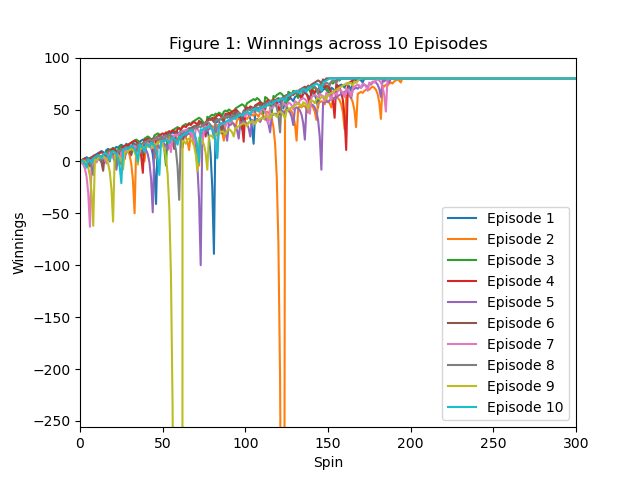
\includegraphics[height=6cm]{Figures/figure1.png}%
\captionof{figure}{This graph shows the winnings recorded after each spin for 10 episodes of simulation.}\label{fig:figure1}%
\end{jdffigure}

In \textbf{Figure 1}, we see that the player reaches \$80 and takes their winnings in all 10 episodes before ever even reaching the 200th spin.
There are streaks of losses that lead to large negative spikes, some of which fall below \$-256 and off the graph, reaching a minimum of \$-8172 in Episode 9. 
Out of all the episodes, the longest it took for a player to reach their goal of \$80 was 195 spins.
Even when there were losing streaks leading to large losses, the player would rapidly recover sooner or later.
This is because whenever the player loses, the next bet is sized to recover all of the player's losses.
Therefore, it only takes one winning spin for the player's profits to recover, no matter how long a losing streak may persist. 

Next, we will analyze statistics for each spin from 1000 episodes.

\begin{jdffigure}
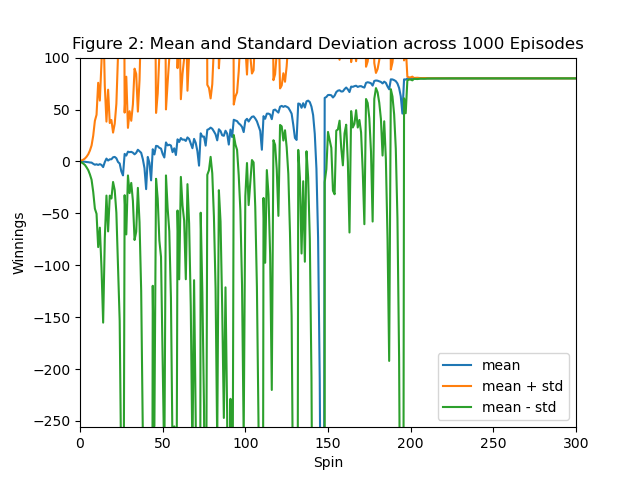
\includegraphics[height=6cm]{Figures/figure2.png}%
\captionof{figure}{This graph shows the mean and standard deviation of winnings for spins across 1000 episodes.}\label{fig:figure2}%
\end{jdffigure}
	
In \textbf{Figure 2}, we can see that the mean, \(mean + std\), and \(mean - std\) all trend towards \$80 as the number of spins increased.
The player tends to reach the the goal of \$80 before spin 200. 
The longest it took for a player to reach an average of \$80 was 214 spins.
While the mean is fairly stable with some large dips, the standard deviation shows much higher volatility. 
The standard deviation lines are consistently far from the mean, and they have numerous spikes stretching well beyond the frames of the graph.
This shows that while all episodes have winnings that trend towards \$80, they contain individual datapoints that vary greatly.

\begin{jdffigure}
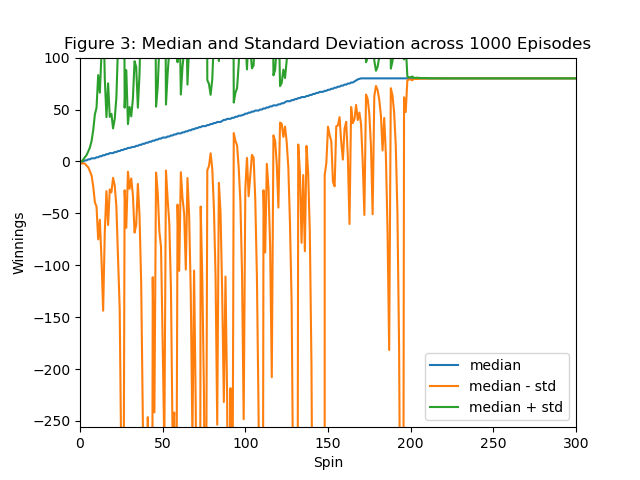
\includegraphics[height=6cm]{Figures/figure3.png}%
\captionof{figure}{This graph shows the median and standard deviation of winnings for spins across 1000 episodes.}\label{fig:figure3}%
\end{jdffigure}

In \textbf{Figure 3}, we see a similar graph that shows the median instead of the mean. 
The median follows the same path to \$80 as the mean, but it is much more stable. 
It reaches the \$80 target at spin 170 and flatlines from there.
While the standard deviation shows us that it will reach quite large values, these anomalies are too rare to affect the median in any significant way.
Because the median is less affected by volatility than the mean, it reaches the goal of \$80 around 30 spins earlier.

Overall, the results of Experiment 1 shows that Profesor Barch's strategy is consistently profitable, within the constraints that the player
stops after winning \$80, and has unlimited funds to continue playing with exponential losses when they hit a losing streak.

\subsection{Experiment 2}
Unforuntately, it is not feasible for most players to assume an unlimited bankroll. *Sigh*. 
Therefor, we will analyze the means and medians of winnings across 1000 episodes again, but with a bankroll of \$256.
If at any point during these spins the player has accrued losses of \$256, they will be forced to stop playing and take their losses.

\begin{jdffigure}
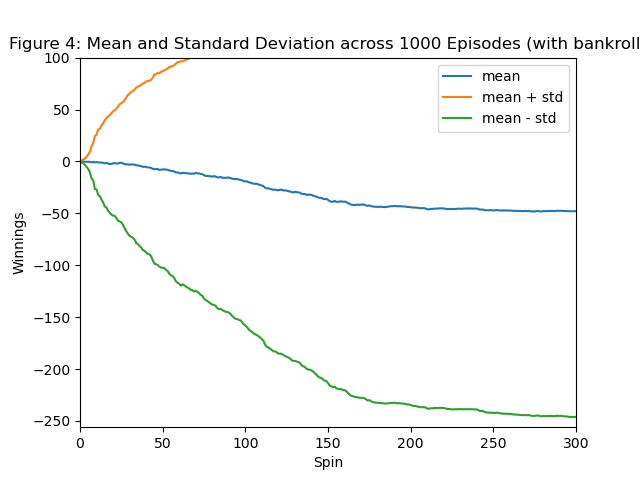
\includegraphics[height=6cm]{Figures/figure4.png}%
\captionof{figure}{This graph shows the mean and standard deviation of winnings for spins across 1000 episodes with a bankroll of \$256.}\label{fig:figure4}%
\end{jdffigure}

\textbf{Figure 4} shows a much different story than the graphs from \emph{Experiment 1}. 
Here, the mean drops below 0 and, instead of being profitable, reaches \$-47.734 at spin 300.
The standard deviation is much more stable than before, but is consistently very large, reaching 198.274 at spin 300.

\begin{jdffigure}
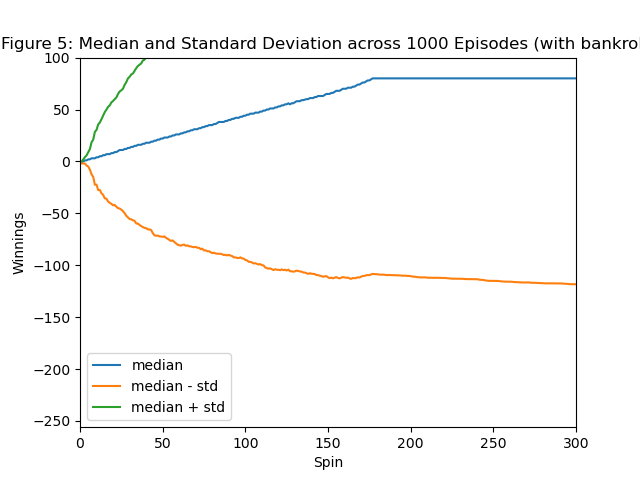
\includegraphics[height=6cm]{Figures/figure5.png}%
\captionof{figure}{This graph shows the median and standard deviation of winnings for spins across 1000 episodes with a bankroll of \$256.}\label{fig:figure5}%
\end{jdffigure}

\textbf{Figure 5}
On the other hand, \textbf{Figure 5} shows the median still approaches \$80.
This tells us that most players are still achieving their goal of \$80 even with a limited bankroll of \$256.
Hoever, the extremely high standard deviation should warn potential gamblers that the potential for losses are very high.
In Experiment 2, 292 / 1000 players were forced to stop playing after losing \$256.

\section{Questions}

\subsection{Question 1} 
Experiment 1 suggests that a player using the strategy can expect to win the \$80 target 100\% of the time
This result can be deduced because the mean and median converge at \$80 in \textbf{Figures 2 \& 3}, and the standard deviation converges at zero.
This means all players in the experiment were successful at reaching the target.

\subsection{Question 2}
In Experiment 1, the expected value of winnings for a player using the strategy is \$80.
This can be calculated by averaging the values of all episodes on their last spin.
In this case, the result is trivial to compute as we already know every episode ended with the player winning \$80.

\subsection{Question 3}
In Experiment 1, \((mean + std)\) and \((mean - std)\) both vary wildly until eventually converging at \$80.
It converges there after all players have reached the target, which is not long after the mean reaches the target.

\subsection{Question 4}
Experiment 2 suggests that a player using the strategy can expect to win the \$80 target 70.8\% of the time.
This is calculated by counting the number of episodes that end with positive winnings (708) and dividing by the number of episodes (1000).

\subsection{Question 5}
In Experiment 2, the expected value of winnings for a player using the strategy is \$-49.892.
This is calcualted by taking the average of every episodes winnings on their final spin.
This shows that with a \$256 bankroll, the player is expected to lose money on average.

\subsection{Question 6}
In Experiment 2, \((mean + std)\) and \((mean - std)\) never converge.
\textbf{Figure 4} shows that the standard deviation grows rapidly until stabilizing somewhere around 200.
It is expected that standard deviation will hit maximums and minimums because the maximum winnings and losses are now bounded from +\$80 to -\$256,
whereas in Experiment 1, the maximum losses were unbounded.

\subsection{Question 7}
It is good to use Expected Value calculated over a large number of episodes to draw conclusions.
This is because as you test more episodes, the results begin to show the distribution of possible outcomes.
Only testing one episode could lead to many different conclusions especially if volatility is high, and will not take into account the diverse range of potential outcomes.
Overall, the expected value shows what someone can "expect" a normal result to look like, although outliers may exist. 
This can be calculated over an endless amount of episodes, and the accuracy of the expectation rises as more episodes are tested.
One episode on it's own provides will not be as accurate as an expected value calcualted over many episodes.

\section{Conclusions}

Profesor Barch's strategy shows promise for winning money, especially based on the results of Experiment 1 with no bankroll.
This shows that eventually, the player has to reach there target as long as they keep playing.
However, once the reality of bankrolls are introduced to the Monte Cristo simulation, the player may no longer be expected to win.
Experiment 2 showed that a player with only \$256 to lose and a target of \$80 will lose money 29.2\% of the time.
While the chances of losing money isn't too bad, the potential for large losses leads to an expected return of -\$49.892.

Although this strategy did not quite work with the target and bankroll we set, further research could be done to find optimal values to lose.
We could expect that raising the bankroll or decreasing the target will increase the chances of being profitable.
It may be possible to find a balance that will lead to a positive expected value of winnings as well.




\end{document}